\documentclass[aspectratio=169,10pt]{beamer}
% =====================================================================
%  Le Collé — thème de présentation (même palette et mêmes notations que la fiche)
% =====================================================================
\usepackage[utf8]{inputenc}
\usepackage[T1]{fontenc}
\usepackage[sc]{mathpazo}
\usepackage[scaled=0.92]{helvet}
\usefonttheme{professionalfonts}
\usepackage{amsmath,amssymb,mathrsfs,stmaryrd}
\usepackage{microtype}
\usepackage{booktabs,array,multicol}
\usepackage[most]{tcolorbox}
\usepackage{tikz,pgfplots}
\usetikzlibrary{arrows.meta,calc,positioning,decorations.pathreplacing,shapes.misc}
\pgfplotsset{compat=1.17,trig format plots=rad}
\usepackage{tkz-tab}

% ---------- palette (identique à la fiche) ----------
\definecolor{Ink}{HTML}{1C2533}\definecolor{Bleu}{HTML}{1F3A5F}\definecolor{BleuMoyen}{HTML}{4A6A8F}
\definecolor{BleuClair}{HTML}{9DB2C9}\definecolor{Fond}{HTML}{F2F4F7}\definecolor{Ocre}{HTML}{B07A26}
\definecolor{Brique}{HTML}{A23B2A}\definecolor{Gris}{HTML}{5E6672}\definecolor{Filet}{HTML}{C5CCD6}
\definecolor{Vert}{HTML}{2E6B4F}

% ---------- notations (identiques à la fiche) ----------
\newcommand{\K}{\mathbb{K}}\newcommand{\R}{\mathbb{R}}\newcommand{\C}{\mathbb{C}}\newcommand{\Z}{\mathbb{Z}}
\newcommand{\Mn}[1]{\mathcal{M}_{n}(#1)}\newcommand{\rg}{\operatorname{rg}}\newcommand{\vect}{\operatorname{Vect}}
\newcommand{\Mat}{\operatorname{Mat}}\newcommand{\Id}{\operatorname{Id}}\newcommand{\com}{\operatorname{com}}
\newcommand{\vv}[1]{\overrightarrow{#1}}\newcommand{\ve}[1]{\vec{#1}}
\newcommand{\dt}[1]{\left|\begin{matrix}#1\end{matrix}\right|}
\DeclareRobustCommand{\HP}{{\sffamily\bfseries\scriptsize\textcolor{Brique}{[HP]}}}

% ---------- réglages beamer ----------
\setbeamertemplate{navigation symbols}{}
\setbeamersize{text margin left=0.85cm,text margin right=0.85cm}
\setbeamercolor{normal text}{fg=Ink,bg=white}
\setbeamercolor{structure}{fg=Bleu}
\setbeamercolor{alerted text}{fg=Brique}
\setbeamerfont{alerted text}{series=\bfseries}
\setbeamertemplate{itemize item}{\raisebox{0.15em}{\textcolor{Ocre}{\rule{0.38em}{0.38em}}}}
\setbeamertemplate{itemize subitem}{\textcolor{BleuMoyen}{\scriptsize\textbullet}}
\setbeamertemplate{enumerate item}{\textcolor{Bleu}{\sffamily\bfseries\insertenumlabel.}}
\setlength{\leftmargini}{1.2em}
\setbeamertemplate{blocks}[default]

% numéro de la partie courante, rappelé dans le titre et le pied de page (renvoi à la fiche)
\def\fichesec{}\def\chapnom{}
\newcommand{\chapitre}[1]{\def\chapnom{#1}}

\setbeamertemplate{frametitle}{%
  \vskip0.28cm
  \ifx\fichesec\empty\else
    \tikz[baseline=(b.base)]\node[fill=Ocre,text=white,font=\sffamily\bfseries\scriptsize,inner sep=2.5pt,rounded corners=1pt](b){\fichesec};\hspace{0.45em}%
  \fi
  {\color{Bleu}\sffamily\bfseries\Large\insertframetitle}\par
  \vskip0.06cm{\color{Filet}\rule{\linewidth}{0.5pt}}\vskip-0.2cm}

\setbeamertemplate{footline}{%
  \hbox to\paperwidth{%
    \hspace*{0.85cm}{\scriptsize\sffamily\color{Gris}Le Collé\ \ \textcolor{Filet}{|}\ \ \chapnom}\hfill
    {\scriptsize\sffamily\color{Gris}\ifx\fichesec\empty\else fiche \textbf{\color{Ocre}§\fichesec}\quad\fi\insertframenumber}\hspace*{0.85cm}}%
  \vskip0.18cm
  \hbox{\begin{tikzpicture}
    \fill[Fond] (0,0) rectangle (\paperwidth,2.2pt);
    \pgfmathsetmacro\prog{min(\insertframenumber/max(\inserttotalframenumber,1),1)}
    \fill[Ocre] (0,0) rectangle ({\prog*\paperwidth},2.2pt);
  \end{tikzpicture}}}

% ---------- encadrés : même code couleur que la fiche ----------
\tcbset{sb/.style={enhanced,arc=1pt,boxrule=0pt,left=6pt,right=6pt,top=3pt,bottom=3pt,before skip=0.14cm,after skip=0.14cm,
  fontupper=\normalsize\raggedright}}
\newcommand{\etiq}[2]{{\sffamily\bfseries\scriptsize\color{#1}\MakeUppercase{#2}}\par\vspace{2pt}}
\newtcolorbox{DEF}[1][Définition]{sb,colback=white,borderline west={2pt}{0pt}{Bleu},before upper={\etiq{Bleu}{#1}}}
\newtcolorbox{PROP}[1][Propriété]{sb,colback=Fond,borderline west={3pt}{0pt}{Bleu},before upper={\etiq{Bleu}{#1}}}
\newtcolorbox{FORM}[1][Formule]{sb,colback=white,colframe=BleuMoyen,boxrule=0.6pt,before upper={\etiq{BleuMoyen}{#1}}}
\newtcolorbox{METH}[1]{sb,colback=white,borderline north={1pt}{0pt}{Bleu},borderline south={1pt}{0pt}{Bleu},
  before upper={{\sffamily\bfseries\scriptsize\colorbox{Bleu}{\color{white}MÉTHODE}\ \color{Bleu}#1}\par\vspace{3pt}}}
\newtcolorbox{PIEGE}[1][Piège]{sb,colback=Brique!6,borderline west={2pt}{0pt}{Brique},before upper={\etiq{Brique}{#1}}}
\newtcolorbox{ASTU}[1][Astuce]{sb,colback=Ocre!8,borderline west={2pt}{0pt}{Ocre},before upper={\etiq{Ocre}{#1}}}
\newtcolorbox{HPBOX}{sb,colback=white,borderline west={2pt}{0pt}{Brique},before upper={\etiq{Brique}{Hors programme}}}
\newtcolorbox{ATOI}[1][À toi]{sb,colback=Vert!6,borderline west={2pt}{0pt}{Vert},before upper={\etiq{Vert}{#1}}}
\newtcolorbox{RETENIR}{sb,colback=Bleu!5,colframe=Bleu,boxrule=0.8pt,left=8pt,
  before upper={\etiq{Bleu}{À retenir}}}
\newtcolorbox{EX}[1][Exemple]{sb,colback=white,colframe=Filet,boxrule=0.5pt,before upper={\etiq{Gris}{#1}}}

% complément pédagogique absent du livre : étiquette pointillée
\DeclareRobustCommand{\ajout}{\tikz[baseline=(a.base)]\node[draw=Gris,dashed,text=Gris,font=\sffamily\scriptsize,inner sep=2pt,rounded corners=1pt](a){complément hors livre};}
\DeclareRobustCommand{\livre}[1]{{\sffamily\scriptsize\color{Gris}[livre #1]}}
\newcommand{\rep}[1]{\textcolor{Vert}{#1}}% réponse attendue de l'élève

% ---------- styles de figures (identiques au livre) ----------
\pgfplotsset{courbe/.style={axis lines=middle,axis equal image,
  axis line style={Gris,-{Stealth[length=4pt]}},
  xlabel={$x$},ylabel={$y$},ticklabel style={font=\scriptsize\sffamily,color=Gris},
  every axis x label/.style={at={(ticklabel* cs:1)},anchor=west,font=\small},
  every axis y label/.style={at={(ticklabel* cs:1)},anchor=south,font=\small},
  samples=200,smooth}}
\pgfplotsset{mini/.style={axis lines=middle,axis line style={Filet},xtick=\empty,ytick=\empty,width=3.9cm,height=3.9cm,
  xmin=-1.15,xmax=1.15,ymin=-1.15,ymax=1.15,title style={font=\footnotesize\sffamily,yshift=-0.1cm},samples=100}}
\tikzset{arcetude/.style={Bleu,line width=1.25pt},
         reste/.style={BleuClair,line width=1pt},
         tgte/.style={Ocre,line width=1pt},
         asy/.style={Gris,dashed,line width=0.7pt},
         pt/.style={circle,fill=Ink,inner sep=1.3pt},
         >={Stealth[length=5pt]}}

% ---------- diapositives de partie ----------
% \partie{num}{titre}{question guide}{liste des parties du chapitre via \rm}
\newcommand{\rmitem}[2]{\def\tmp{#1}%
  \ifx\tmp\fichesec{\color{Bleu}\bfseries #1\quad #2}\else{\color{Gris!70}#1\quad #2}\fi\par\vspace{2pt}}
\newcommand{\partie}[4]{%
  \def\fichesec{#1}\section{#2}%
  \begin{frame}[plain]
  \begin{tikzpicture}[remember picture,overlay]
    \fill[Bleu] (current page.north west) rectangle ([xshift=6.3cm]current page.south west);
    \node[anchor=north west,text=white,font=\sffamily\bfseries\fontsize{40}{40}\selectfont] at ([xshift=0.8cm,yshift=-1.2cm]current page.north west) {#1};
    \node[anchor=north west,text width=4.8cm,align=left,text=white,font=\sffamily\bfseries\Large] at ([xshift=0.8cm,yshift=-2.9cm]current page.north west) {\hyphenpenalty=10000\exhyphenpenalty=10000 #2\par};
    \node[anchor=south west,text width=4.8cm,text=white!75!Bleu,font=\sffamily\scriptsize] at ([xshift=0.8cm,yshift=0.6cm]current page.south west) {\chapnom\\fiche \textbf{§#1}};
  \end{tikzpicture}
  \hspace*{5.5cm}\begin{minipage}{8.4cm}
  {\sffamily\scriptsize\color{Ocre}\bfseries LA QUESTION}\par\vspace{2pt}
  {\large #3}\par\vspace{0.7cm}
  {\sffamily\scriptsize\color{Gris}\bfseries DANS CE CHAPITRE}\par\vspace{4pt}
  {\sffamily\small #4}
  \end{minipage}
  \end{frame}}



% ---------- exercices en séance : énoncé sur une diapositive, correction sur la suivante ----------
\newcommand{\badgeexo}[1]{\tikz[baseline=(e.base)]\node[fill=Vert,text=white,font=\sffamily\bfseries\scriptsize,inner sep=2.5pt,rounded corners=1pt](e){EXERCICE #1};\hspace{0.4em}}
\newcommand{\badgecor}[1]{\tikz[baseline=(e.base)]\node[draw=Vert,line width=0.8pt,text=Vert,font=\sffamily\bfseries\scriptsize,inner sep=2.2pt,rounded corners=1pt](e){CORRECTION #1};\hspace{0.4em}}
\newtcolorbox{ENONCE}[1][]{sb,colback=Vert!6,borderline west={3pt}{0pt}{Vert},left=9pt,top=5pt,bottom=5pt,
  before upper={{\sffamily\bfseries\scriptsize\color{Vert}À TOI\ifx\relax#1\relax\else\ \ ·\ \ \MakeUppercase{#1}\fi}\par\vspace{4pt}}}
\newtcolorbox{INDICE}{sb,colback=white,colframe=Vert!60,boxrule=0.5pt,borderline={0.5pt}{0pt}{Vert!60,dashed},
  before upper={\etiq{Vert}{Indice (si besoin)}}}
\newtcolorbox{RAIS}[1][Le raisonnement]{sb,colback=Vert!5,borderline west={2pt}{0pt}{Vert},before upper={\etiq{Vert}{#1}}}
\newtcolorbox{OUTIL}{sb,colback=Fond,borderline west={2pt}{0pt}{Bleu},before upper={\etiq{Bleu}{Propriété ou méthode utilisée}}}
\newcommand{\etape}[1]{{\sffamily\bfseries\footnotesize\color{Vert}#1}\ }
\newcommand{\objectif}[1]{\par\vspace{2pt}{\footnotesize\sffamily\color{Gris}Objectif : #1}}
\newcommand{\Ker}{\operatorname{Ker}}\renewcommand{\Im}{\operatorname{Im}}\newcommand{\tr}{\operatorname{tr}}\newcommand{\Sp}{\operatorname{Sp}}
\newcommand{\GLn}[1]{\mathrm{GL}_n(#1)}
\providecommand{\N}{\mathbb{N}}\providecommand{\ch}{\operatorname{ch}}\providecommand{\sh}{\operatorname{sh}}
\title{Le Collé --- Séries entières}

\begin{document}

% ---------------------------------------------------------------- titre
\begin{frame}[plain]
\begin{tikzpicture}[remember picture,overlay]
  \fill[Bleu] (current page.north west) rectangle (current page.south east);
  \node[anchor=north west,text=white!70!Bleu,font=\sffamily\scriptsize] at ([xshift=1cm,yshift=-1.2cm]current page.north west)
    {LE COLLÉ\ \ ·\ \ MATHÉMATIQUES PT\ \ ·\ \ CHAPITRE 8\ \ ·\ \ SUPPORT DE SÉANCE};
  \node[anchor=north west,text=white,font=\sffamily\bfseries\fontsize{26}{30}\selectfont,text width=13cm] at ([xshift=1cm,yshift=-2.1cm]current page.north west)
    {Séries entières};
  \fill[Ocre] ([xshift=1cm,yshift=-4.6cm]current page.north west) rectangle ([xshift=4cm,yshift=-4.65cm]current page.north west);
  \node[anchor=north west,text=white!80!Bleu,font=\normalsize,text width=12.5cm] at ([xshift=1cm,yshift=-5cm]current page.north west)
    {Présentation pour expliquer, avec six exercices à chercher en séance ;\\ le \textbf{livret} pour relire, la \textbf{fiche} pour réviser.
     Mêmes parties (§1.1 à §1.7), mêmes notations.};
\end{tikzpicture}
\end{frame}

% ---------------------------------------------------------------- plan
\begin{frame}{Plan : trois séances de 2 h}
\begin{columns}[T]
\column{0.58\textwidth}
\small
\renewcommand{\arraystretch}{1.25}
\begin{tabular}{@{}l l r@{}}
\multicolumn{3}{@{}l}{\sffamily\bfseries\color{Ocre}Séance 1 --- Taylor et rayon}\\
\textbf{\color{Bleu}1.1} & Série de Taylor d'une fonction & \color{Vert}Ex.~1\\
\textbf{\color{Bleu}1.2} & Séries entières, rayon & \\
\textbf{\color{Bleu}1.3} & Calcul du rayon & \color{Vert}Ex.~2, 3\\[2pt]
\multicolumn{3}{@{}l}{\sffamily\bfseries\color{Ocre}Séance 2 --- la fonction somme}\\
\textbf{\color{Bleu}1.4} & Continuité, dérivation, intégration & \color{Vert}Ex.~4\\
\textbf{\color{Bleu}1.5} & Fonctions DSE, DSE usuels & \\[2pt]
\multicolumn{3}{@{}l}{\sffamily\bfseries\color{Ocre}Séance 3 --- développer}\\
\textbf{\color{Bleu}1.6} & Méthodes de développement & \color{Vert}Ex.~5, 6\\
\textbf{\color{Bleu}1.7} & Synthèse &
\end{tabular}
\column{0.38\textwidth}
\begin{ASTU}[Le fil du chapitre]
\small Écrire une fonction comme un \textbf{polynôme de degré infini} $a_0+a_1x+a_2x^2+\cdots$\\[3pt]
Deux questions : \textbf{pour quels $x$} ? et \textbf{quelles fonctions} ?
\end{ASTU}
{\small\color{Gris}Prérequis : séries numériques (ch.~7), Taylor (PTSI), équations différentielles (ch.~4).}
\end{columns}
\end{frame}

\chapitre{Chapitre 8 · Séries entières}
\newcommand{\rmI}{\rmitem{1.1}{Série de Taylor}\rmitem{1.2}{Rayon de convergence}\rmitem{1.3}{Calcul du rayon}
  \rmitem{1.4}{Fonction somme}\rmitem{1.5}{Fonctions DSE}\rmitem{1.6}{Développer}\rmitem{1.7}{Synthèse}}

\begin{frame}{Le problème : un polynôme de degré infini}
\begin{columns}[T]
\column{0.5\textwidth}
Pour $|x|<1$ : $\displaystyle\frac1{1-x}=1+x+x^2+x^3+\cdots$\\[6pt]
\pause
Les sommes partielles $1+x+\dots+x^n$ sont des polynômes qui \textbf{approchent} $\frac1{1-x}$\dots\\[4pt]
\pause
\dots\ mais seulement pour $|x|<1$ : au-delà, la somme n'a plus de sens.
\column{0.46\textwidth}
\centering
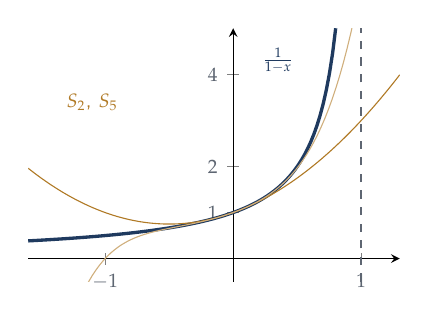
\begin{tikzpicture}
\begin{axis}[width=6.3cm,height=4.8cm,axis lines=middle,xmin=-1.6,xmax=1.3,ymin=-0.5,ymax=5,
  ticklabel style={font=\scriptsize\sffamily,color=Gris},xtick={-1,1},ytick={1,2,4},samples=100]
\addplot[Bleu,line width=1.2pt,domain=-1.6:0.8] {1/(1-x)};
\addplot[Ocre,domain=-1.6:1.3] {1+x+x^2};
\addplot[Ocre!60,domain=-1.6:1.3] {1+x+x^2+x^3+x^4+x^5};
\addplot[asy,domain=-0.5:5] coordinates {(1,-0.5)(1,5)};
\node[font=\scriptsize\sffamily,Bleu] at (axis cs:0.35,4.3) {$\frac1{1-x}$};
\node[font=\scriptsize\sffamily,Ocre] at (axis cs:-1.1,3.4) {$S_2$, $S_5$};
\end{axis}
\end{tikzpicture}
\end{columns}
\pause
\begin{RETENIR}
Deux questions : \textbf{pour quels $x$} la série $\sum a_nx^n$ converge-t-elle (le \textbf{rayon}) ;
\textbf{quelles fonctions} s'écrivent ainsi (les \textbf{DSE}).
\end{RETENIR}
\end{frame}

% =====================================================================
\partie{1.1}{Série de Taylor d'une fonction}{Une fonction très régulière est-elle la somme de sa série de Taylor ?}{\rmI}

\begin{frame}{Formule de Taylor avec reste intégral}
\begin{PROP}[Théorème \livre{th.~1.1}]
$f$ de classe $\mathcal C^{n+1}$ sur $I\ni0$ : pour tout $x\in I$,
\[f(x)=\sum_{k=0}^n\frac{f^{(k)}(0)}{k!}x^k+\underbrace{\int_0^x\frac{(x-t)^n}{n!}f^{(n+1)}(t)\,dt}_{R_n(x)}.\]
\end{PROP}
\pause
\begin{columns}[T]
\column{0.5\textwidth}
\begin{EX}[Démonstration]
Récurrence ; $n=0$ : $f(x)=f(0)+\int_0^xf'$.\\
Hérédité : intégration par parties du reste, avec $v(t)=-\frac{(x-t)^n}{n!}$.
\end{EX}
\column{0.46\textwidth}
\begin{PROP}[Taylor-Lagrange \livre{cor.~1.2}]
$|f^{(n+1)}|\leq M$ : $|R_n(x)|\leq M\frac{|x|^{n+1}}{(n+1)!}$.
\end{PROP}
\end{columns}
\end{frame}

\begin{frame}{Série de Taylor}
\begin{DEF}[Définition \livre{déf.~1.3}]
$f$ de classe $\mathcal C^\infty$ près de $0$ : la \emph{série de Taylor} de $f$ est $\displaystyle\sum\frac{f^{(n)}(0)}{n!}x^n$.
\end{DEF}
\pause
Ses sommes partielles sont $f(x)-R_n(x)$. Donc :
\begin{RETENIR}
$f(x)$ est la somme de sa série de Taylor \textbf{si et seulement si} $R_n(x)\to0$.
\end{RETENIR}
\pause
\begin{PIEGE}
Ce n'est pas automatique : $f(x)=e^{-1/x^2}$ ($f(0)=0$) a toutes ses dérivées nulles en $0$. Sa série de Taylor est nulle, $f$ ne l'est pas.
\end{PIEGE}
\end{frame}

\begin{frame}{La série exponentielle}
\begin{PROP}[Théorème \livre{th.~1.4}]
Pour tout $x\in\R$ : $\displaystyle e^x=\sum_{n=0}^{+\infty}\frac{x^n}{n!}$.
\end{PROP}
\pause
\begin{columns}[T]
\column{0.56\textwidth}
\etape{Preuve.} $R_n(x)=\int_0^x\frac{(x-t)^n}{n!}e^t\,dt$ ; on pose $t=xu$ :
\[|R_n(x)|\leq\frac{|x|^{n+1}}{n!}e^{|x|}\!\int_0^1\!(1-u)^n\,du=e^{|x|}\frac{|x|^{n+1}}{(n+1)!}\]
$\to0$
(croissances comparées).
\column{0.4\textwidth}
\pause
\begin{EX}[Calcul de $e$]
$e=\sum\frac1{n!}$, erreur $\leq\frac3{(n+1)!}$.\\
$n=8$ : $\frac3{9!}<10^{-5}$ ;\\ $e\approx2{,}71828$.
\end{EX}
\end{columns}
\end{frame}

\begin{frame}{La famille exponentielle}
\begin{FORM}[Pour tout $x\in\R$ \livre{th.~1.6}]
$\displaystyle\cos x=\sum_{p=0}^{+\infty}\frac{(-1)^px^{2p}}{(2p)!}$,\qquad $\displaystyle\sin x=\sum_{p=0}^{+\infty}\frac{(-1)^px^{2p+1}}{(2p+1)!}$,\\[4pt]
$\displaystyle\ch x=\sum_{p=0}^{+\infty}\frac{x^{2p}}{(2p)!}$,\qquad $\displaystyle\sh x=\sum_{p=0}^{+\infty}\frac{x^{2p+1}}{(2p+1)!}$.
\end{FORM}
\pause
\begin{columns}[T]
\column{0.5\textwidth}
\begin{EX}[Pourquoi]
$\cos^{(k)}(x)=\cos(x+k\frac\pi2)$ : dérivées en $0$ : $1,0,-1,0,\dots$, toutes majorées par $1$ : Taylor-Lagrange.\\
$\ch=\frac{e^x+e^{-x}}2$ : termes pairs.
\end{EX}
\column{0.46\textwidth}
\begin{ASTU}[Mémo]
$\ch$ : termes pairs de $e^x$ ;\ $\sh$ : impairs.\\
$\cos$, $\sin$ : mêmes termes, signes alternés.
\end{ASTU}
\end{columns}
\end{frame}

\begin{frame}{Méthode : sommes avec des factorielles}
\small
\begin{METH}{Famille exponentielle \livre{méth.~1.1}}
1. \textbf{Factoriser} la puissance de $x$ en trop.\quad 2. \textbf{Changer d'indice} pour retrouver $\frac{x^k}{k!}$.\\
3. Polynôme en $n$ : base $n(n-1)$, $n$, $1$, car $\frac{n(n-1)}{n!}=\frac1{(n-2)!}$.\quad 4. Devant $(2n)!$ : $x=t^2$ ou $x=-t^2$.
\end{METH}
\pause
\begin{EX}
$\displaystyle\sum_{n=1}^{+\infty}\frac{x^{n+2}}{(n-1)!}=x^3\sum_{n=1}^{+\infty}\frac{x^{n-1}}{(n-1)!}\overset{k=n-1}{=}x^3\sum_{k=0}^{+\infty}\frac{x^k}{k!}=x^3e^x$.
\end{EX}
\pause
\begin{EX}
$\sum_{n\geq0}\frac{(-1)^nx^n}{(2n+1)!}$ : pour $x=t^2>0$, $\frac1t\sum\frac{(-1)^nt^{2n+1}}{(2n+1)!}=\frac{\sin t}t=\frac{\sin\sqrt x}{\sqrt x}$ ;
pour $x=-t^2<0$ : $\frac{\sh\sqrt{-x}}{\sqrt{-x}}$.
\end{EX}
\end{frame}

\begin{frame}{\badgeexo{1}Sommes de la famille exponentielle}
\begin{ENONCE}[8 min]
Calculer, pour $x\in\R$ :\quad
(a) $\displaystyle\sum_{n=0}^{+\infty}\frac{n^2}{n!}$\qquad (b) $\displaystyle\sum_{n=0}^{+\infty}\frac{n+1}{n!}x^n$\qquad (c) $\displaystyle\sum_{n=0}^{+\infty}\frac{x^{4n}}{(4n)!}$.
\objectif{reconnaître $e^x$, $\ch$, $\cos$ après factorisation et changement d'indice.}
\end{ENONCE}
\pause
\begin{INDICE}
(a) $n^2=n(n-1)+n$.\quad (c) Combiner $\ch x$ et $\cos x$.
\end{INDICE}
\end{frame}

\begin{frame}{\badgecor{1}Sommes de la famille exponentielle}
\begin{columns}[T]
\column{0.36\textwidth}
\begin{RAIS}
On fait apparaître exactement $\frac{x^k}{k!}$ : on simplifie $n$ avec $n!$, puis on décale l'indice.
\end{RAIS}
\column{0.61\textwidth}
\etape{(a)} $\frac{n^2}{n!}=\frac1{(n-2)!}+\frac1{(n-1)!}$ (pour $n\geq2$, $n\geq1$) : somme $e+e=2e$.\\[4pt]
\pause
\etape{(b)} $\frac{n+1}{n!}x^n=\frac{x^n}{(n-1)!}+\frac{x^n}{n!}$ : $xe^x+e^x=(x+1)e^x$.\\[4pt]
\pause
\etape{(c)} Dans $\frac{\ch x+\cos x}2$, le terme $\frac{x^{2p}}{(2p)!}$ a le coefficient $\frac{1+(-1)^p}2$ : il reste $p$ pair.
Somme : $\frac{\ch x+\cos x}2$.
\end{columns}
\end{frame}

% =====================================================================
\partie{1.2}{Séries entières, rayon de convergence}{Pour quels $z$ la série $\sum a_nz^n$ converge-t-elle ?}{\rmI}

\begin{frame}{Série entière, lemme d'Abel}
\begin{DEF}[Définition \livre{déf.~1.8}]
Une \emph{série entière} est une série $\sum a_nz^n$, de coefficients $a_n\in\K$, de variable $z$ réelle ou complexe.
\end{DEF}
\pause
\begin{PROP}[Lemme d'Abel \livre{prop.~1.10}]
Si $(a_nz_0^n)$ est \textbf{bornée}, alors $\sum a_nz^n$ converge absolument pour tout $|z|<|z_0|$.
\end{PROP}
\pause
\begin{EX}[Preuve]
$|a_nz^n|=|a_nz_0^n|\cdot\left|\frac z{z_0}\right|^n\leq M\left|\frac z{z_0}\right|^n$ : comparaison avec une série géométrique de raison $<1$.
\end{EX}
\end{frame}

\begin{frame}{Le rayon de convergence}
\begin{DEF}[Définition \livre{déf.~1.11}]
$R=\sup\{r\geq0:(a_nr^n)\text{ est bornée}\}\in[0,+\infty]$.
\end{DEF}
\pause
\begin{columns}[T]
\column{0.55\textwidth}
\begin{PROP}[Théorème \livre{th.~1.12}]
\textbullet\ $|z|<R$ : convergence \textbf{absolue}.\\
\textbullet\ $|z|>R$ : divergence \textbf{grossière}.\\
\textbullet\ $|z|=R$ : \textbf{on ne sait pas}.
\end{PROP}
\column{0.41\textwidth}
\centering
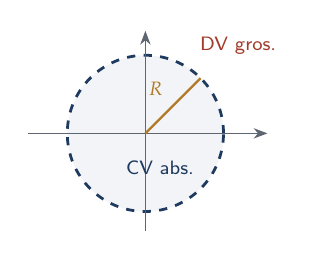
\begin{tikzpicture}[scale=0.62]
\fill[Fond] (0,0) circle (1.6);
\draw[Bleu,line width=1pt,dashed] (0,0) circle (1.6);
\draw[Gris,->] (-2.4,0)--(2.5,0); \draw[Gris,->] (0,-2)--(0,2.1);
\draw[Ocre,line width=0.8pt] (0,0)--(1.13,1.13) node[midway,above left,font=\scriptsize,Ocre]{$R$};
\node[font=\scriptsize\sffamily,Bleu] at (0.3,-0.7) {CV abs.};
\node[font=\scriptsize\sffamily,Brique] at (1.9,1.8) {DV gros.};
\end{tikzpicture}
\end{columns}
\pause
\begin{EX}[Au bord, tout peut arriver]
$\sum z^n$, $\sum\frac{z^n}n$, $\sum\frac{z^n}{n^2}$ : $R=1$. En $z=1$ : DV, DV, CV. En $z=-1$ : DV, CV, CV.
\end{EX}
\end{frame}

\begin{frame}{Encadrer le rayon}
\begin{PROP}[Proposition \livre{prop.~1.15}]
$\sum a_nz_0^n$ converge $\Rightarrow R\geq|z_0|$.\quad Diverge $\Rightarrow R\leq|z_0|$.\quad CV \textbf{non absolue} $\Rightarrow R=|z_0|$.
\end{PROP}
\pause
\begin{columns}[T]
\column{0.5\textwidth}
\begin{EX}
$\sum\frac{(-1)^n}n$ converge, pas absolument : $\sum\frac{z^n}n$ a pour rayon $1$.
\end{EX}
\column{0.46\textwidth}
\begin{EX}
CV en $\sqrt2\,i$, DV en $1+i$ : $\sqrt2\leq R\leq\sqrt2$, donc $R=\sqrt2$.
\end{EX}
\end{columns}
\pause
\begin{PIEGE}
Le rayon ne dit \textbf{rien} au bord : la nature en $x=\pm R$ s'étudie avec les séries numériques.
\end{PIEGE}
\end{frame}

% =====================================================================
\partie{1.3}{Calcul du rayon de convergence}{Comment trouver $R$ sans revenir à la définition ?}{\rmI}

\begin{frame}{Comparaison et équivalents}
\begin{columns}[T]
\column{0.5\textwidth}
\begin{PROP}[Comparaison \livre{prop.~1.17}]
$|a_n|\leq|b_n|$ à partir d'un rang $\Rightarrow R_a\geq R_b$.
\end{PROP}
\column{0.46\textwidth}
\begin{PROP}[Équivalents \livre{prop.~1.18}]
$|a_n|\sim|b_n|\Rightarrow R_a=R_b$.
\end{PROP}
\end{columns}
\pause
\begin{EX}
$\sum\sin(n)z^n$ : $|\sin n|\leq1$ donne $R\geq1$ ; en $z=1$, $\sin n\not\to0$ : DV, donc $R\leq1$. \textbf{$R=1$}.
\end{EX}
\pause
\begin{EX}
$\sum\left(\frac\pi2-\arctan n\right)z^n$ : $\frac\pi2-\arctan n=\arctan\frac1n\sim\frac1n$ : comme $\sum\frac{z^n}n$, \textbf{$R=1$}.
\end{EX}
\end{frame}

\begin{frame}{La règle de d'Alembert}
\begin{METH}{Rayon par d'Alembert \livre{méth.~1.2}}
Sur la série \textbf{numérique} $\sum|a_nz^n|$, $z\neq0$ : $\dfrac{|a_{n+1}|}{|a_n|}|z|\to L|z|$.\quad
$L|z|<1$ : CV ; $L|z|>1$ : DV.\quad Donc $R=\frac1L$.
\end{METH}
\pause
\begin{columns}[T]
\column{0.5\textwidth}
\begin{EX}
$\sum\frac{z^n}{n!}$ : $\frac{|z|}{n+1}\to0$ : $R=+\infty$.\\
$\sum n^nz^n$ : $(n+1)(1+\frac1n)^n|z|\to+\infty$ : $R=0$.
\end{EX}
\column{0.46\textwidth}
\begin{PIEGE}[Série lacunaire]
$\sum\frac{x^{2n}}n$ : $a_{2p+1}=0$, pas de quotient $\frac{a_{n+1}}{a_n}$. Quotient des termes \textbf{présents} : $\frac n{n+1}x^2\to x^2$ : $R=1$.
\end{PIEGE}
\end{columns}
\end{frame}

\begin{frame}{Même rayon, somme, produit de Cauchy}
\begin{PROP}[\livre{prop.~1.21}]
$\sum a_nz^n$ et $\sum n^\alpha a_nz^n$ ont le \textbf{même rayon} ; $\sum n^\alpha z^n$ : $R=1$.
\end{PROP}
\pause
\begin{columns}[T]
\column{0.48\textwidth}
\begin{PROP}[Somme \livre{prop.~1.22}]
$R\geq\min(R_a,R_b)$, égalité si $R_a\neq R_b$.
\end{PROP}
\column{0.48\textwidth}
\begin{PROP}[Produit de Cauchy \livre{th.~1.23}]
$c_n=\sum_{k=0}^na_kb_{n-k}$ : $R\geq\min$ et la somme est le produit.
\end{PROP}
\end{columns}
\pause
\begin{EX}
$\sum z^n\cdot\sum z^n$ : $c_n=n+1$, donc $\displaystyle\frac1{(1-z)^2}=\sum_{n=0}^{+\infty}(n+1)z^n$ pour $|z|<1$.
\end{EX}
\end{frame}

\begin{frame}{\badgeexo{2}Rayons de convergence}
\begin{ENONCE}[10 min]
Rayon de :\quad (a) $\sum e^{\cos n}z^n$\quad (b) $\sum\frac{e^{in}}{1+in}z^n$\quad (c) $\sum\frac{(2n)!}{(n!)^2}z^n$\quad (d) $\sum\frac{(-1)^n}{n(n-1)}z^n$.
\objectif{choisir l'outil : comparaison, équivalent, d'Alembert.}
\end{ENONCE}
\pause
\begin{INDICE}
(a) encadrer $e^{\cos n}$.\quad (b) calculer le module.\quad (c) d'Alembert.
\end{INDICE}
\end{frame}

\begin{frame}{\badgecor{2}Rayons de convergence}
\begin{columns}[T]
\column{0.36\textwidth}
\begin{RAIS}
On lit la forme du coefficient : borné, équivalent simple, ou factorielles.
\end{RAIS}
\column{0.61\textwidth}
\etape{(a)} $e^{-1}\leq e^{\cos n}\leq e$ : $1\leq R\leq1$, \textbf{$R=1$}.\\[3pt]
\pause
\etape{(b)} $\left|\frac{e^{in}}{1+in}\right|=\frac1{\sqrt{1+n^2}}\sim\frac1n$ : \textbf{$R=1$}.\\[3pt]
\pause
\etape{(c)} $\frac{a_{n+1}}{a_n}=\frac{(2n+2)(2n+1)}{(n+1)^2}\to4$ : \textbf{$R=\frac14$}.\\[3pt]
\pause
\etape{(d)} $\sim\frac1{n^2}$, même rayon que $\sum\frac{z^n}{n^2}$ : \textbf{$R=1$}.
\end{columns}
\end{frame}

\begin{frame}{\badgeexo{3}Rayon et bord}
\begin{ENONCE}[8 min]
1. Rayon de $\sum2^nz^{3n}$.\qquad 2. Rayon de $\sum\frac{x^n}{\sqrt n}$, et nature en $x=1$ et $x=-1$.
\objectif{traiter une série lacunaire ; séparer rayon et bord.}
\end{ENONCE}
\pause
\begin{INDICE}
1. Quotient de deux termes consécutifs \textbf{présents}.\quad 2. Au bord : Riemann, séries alternées.
\end{INDICE}
\end{frame}

\begin{frame}{\badgecor{3}Rayon et bord}
\begin{columns}[T]
\column{0.36\textwidth}
\begin{RAIS}
Le rayon se trouve avec d'Alembert ; le bord, avec les séries numériques.
\end{RAIS}
\column{0.61\textwidth}
\etape{1.} $\frac{|2^{n+1}z^{3n+3}|}{|2^nz^{3n}|}=2|z|^3$ : CV si $2|z|^3<1$, DV si $>1$ : \textbf{$R=2^{-1/3}$}.\\[4pt]
\pause
\etape{2.} $\sqrt{\frac n{n+1}}|x|\to|x|$ : \textbf{$R=1$}.\\
En $1$ : $\sum\frac1{\sqrt n}$ \textbf{DV} (Riemann).\\
En $-1$ : $\sum\frac{(-1)^n}{\sqrt n}$ \textbf{CV} (séries alternées).
\end{columns}
\end{frame}

% =====================================================================
\partie{1.4}{Fonction somme d'une série entière réelle}{Que peut-on faire avec $f(x)=\sum a_nx^n$ ?}{\rmI}

\begin{frame}{Continuité, dérivation}
\begin{PROP}[{Sur $]-R,R[$ \livre{th.~1.27, 1.29}}]
$f(x)=\sum_{n=0}^{+\infty}a_nx^n$ est continue, dérivable, et $\displaystyle f'(x)=\sum_{n=1}^{+\infty}na_nx^{n-1}$ (même rayon).
\end{PROP}
\pause
\begin{PROP}[Classe $\mathcal C^\infty$ \livre{cor.~1.30}]
$f\in\mathcal C^\infty(]-R,R[)$ et $\displaystyle a_p=\frac{f^{(p)}(0)}{p!}$.
\end{PROP}
\pause
\begin{PROP}[Au bord, admis \livre{prop.~1.28}]
Si $\sum a_nR^n$ converge : $\sum a_nR^n=\lim_{x\to R^-}f(x)$ (théorème d'Abel radial).
\end{PROP}
\end{frame}

\begin{frame}{Intégration terme à terme}
\begin{PROP}[Théorème \livre{th.~1.31}]
Pour $x\in\,]-R,R[$ : $\displaystyle\int_0^x\sum_{n=0}^{+\infty}a_nt^n\,dt=\sum_{n=0}^{+\infty}\frac{a_n}{n+1}x^{n+1}$ (même rayon).
\end{PROP}
\pause
\begin{EX}[À partir de $\frac1{1-x}=\sum x^n$]
\textbullet\ dériver : $\sum_{n\geq1}nx^n=\frac x{(1-x)^2}$ ;\\
\textbullet\ intégrer : $-\ln(1-x)=\sum_{n\geq1}\frac{x^n}n$ ;\\
\textbullet\ au bord : $\sum\frac{(-1)^n}n$ converge, donc $\sum_{n\geq1}\frac{(-1)^n}n=\lim_{x\to-1}\big(-\ln(1-x)\big)=-\ln2$.
\end{EX}
\pause
\begin{PIEGE}
Dériver change le bord : $\sum\frac{x^n}{n^2}$ CV en $1$, sa dérivée $\sum\frac{x^{n-1}}n$ DV en $1$.
\end{PIEGE}
\end{frame}

\begin{frame}{Méthode : calculer une somme}
\begin{METH}{Somme d'une série entière \livre{méth.~1.4}}
1. Le \textbf{rayon}. 2. $P(n)x^n$ : dériver $\frac1{1-x}$ ; $P(n)$ sur la base $(n+1)(n+2)$, $n+1$, $1$.\\
3. $\frac{x^n}{n+k}$, fraction : \textbf{intégrer}, éléments simples.\quad 4. $n!$ : famille exponentielle.\quad 5. Contrôler en $0$.
\end{METH}
\pause
\begin{EX}
$n^2=(n+1)(n+2)-3(n+1)+1$ et $\sum(n+1)(n+2)x^n=\left(\frac1{1-x}\right)''=\frac2{(1-x)^3}$ :
\[\sum_{n=0}^{+\infty}n^2x^n=\frac2{(1-x)^3}-\frac3{(1-x)^2}+\frac1{1-x}=\frac{x(1+x)}{(1-x)^3}.\]
\end{EX}
\end{frame}

\begin{frame}{\badgeexo{4}Calculer une somme}
\begin{ENONCE}[10 min]
Rayon et somme de $\displaystyle\sum_{n\geq1}\frac{x^n}{n(n+1)}$. En déduire $\displaystyle\sum_{n=1}^{+\infty}\frac1{n(n+1)2^n}$.
\objectif{éléments simples, puis intégration de la série géométrique.}
\end{ENONCE}
\pause
\begin{INDICE}
$\frac1{n(n+1)}=\frac1n-\frac1{n+1}$ ; et $\sum_{n\geq1}\frac{x^n}{n+1}=\frac1x\sum_{k\geq2}\frac{x^k}k$.
\end{INDICE}
\end{frame}

\begin{frame}{\badgecor{4}Calculer une somme}
\begin{columns}[T]
\column{0.36\textwidth}
\begin{RAIS}
Chaque morceau se ramène à $\sum\frac{x^k}k=-\ln(1-x)$, obtenue en intégrant $\frac1{1-x}$.
\end{RAIS}
\column{0.61\textwidth}
\etape{1.} $R=1$ (d'Alembert).\\[3pt]
\pause
\etape{2.} Pour $0<|x|<1$ : $\sum\frac{x^n}n=-\ln(1-x)$, $\sum\frac{x^n}{n+1}=\frac{-\ln(1-x)-x}x$.\\[3pt]
\pause
\etape{3.} $S(x)=1+\dfrac{(1-x)\ln(1-x)}x$, et $S(0)=0$.\\[3pt]
\pause
\etape{4.} $x=\frac12$ : $\displaystyle\sum_{n=1}^{+\infty}\frac1{n(n+1)2^n}=1-\ln2$.
\end{columns}
\end{frame}

% =====================================================================
\partie{1.5}{Fonctions développables en série entière}{Quelles fonctions s'écrivent comme une série entière ?}{\rmI}

\begin{frame}{DSE : définition, unicité}
\begin{DEF}[Définition \livre{déf.~1.34}]
$f$ est \emph{DSE} sur $]-r,r[$ s'il existe $\sum a_nx^n$ de rayon $R\geq r$ avec $f(x)=\sum a_nx^n$ sur $]-r,r[$.
\end{DEF}
\pause
\begin{PROP}[Le DSE est la série de Taylor \livre{th.~1.35}]
$f$ DSE $\Rightarrow$ $f$ est $\mathcal C^\infty$ et $f(x)=\sum\frac{f^{(n)}(0)}{n!}x^n$ : le DSE est \textbf{unique}.
\end{PROP}
\pause
\begin{columns}[T]
\column{0.48\textwidth}
\begin{PROP}[Parité \livre{prop.~1.36}]
Paire : puissances paires ;\ impaire : impaires.
\end{PROP}
\column{0.48\textwidth}
\begin{PIEGE}
Réciproque fausse : $e^{-1/x^2}$ est $\mathcal C^\infty$, pas DSE.
\end{PIEGE}
\end{columns}
\end{frame}

\begin{frame}{Les DSE usuels}
\small
\begin{columns}[T]
\column{0.48\textwidth}
\begin{FORM}[$R=+\infty$]
$e^x=\sum\frac{x^n}{n!}$\\
$\ch x=\sum\frac{x^{2n}}{(2n)!}$,\ $\sh x=\sum\frac{x^{2n+1}}{(2n+1)!}$\\
$\cos x=\sum\frac{(-1)^nx^{2n}}{(2n)!}$\\
$\sin x=\sum\frac{(-1)^nx^{2n+1}}{(2n+1)!}$
\end{FORM}
\column{0.48\textwidth}
\begin{FORM}[$R=1$ \livre{th.~1.37, 1.38}]
$\frac1{1-x}=\sum x^n$,\ $\frac1{1+x}=\sum(-1)^nx^n$\\
$\ln(1+x)=\sum_{n\geq1}\frac{(-1)^{n+1}}nx^n$\\
$\arctan x=\sum\frac{(-1)^n}{2n+1}x^{2n+1}$\\
$(1+x)^\alpha=1+\sum_{n\geq1}\frac{\alpha(\alpha-1)\cdots(\alpha-n+1)}{n!}x^n$
\end{FORM}
\end{columns}
\pause
\begin{EX}[D'où viennent-ils ?]
$\ln(1+x)$ : intégrer $\frac1{1+t}$.\quad $\arctan$ : intégrer $\frac1{1+t^2}=\sum(-1)^nt^{2n}$.\quad $(1+x)^\alpha$ : équation $(1+x)y'=\alpha y$.\quad
$\C$ : $e^z=\sum\frac{z^n}{n!}$ \livre{th.~1.40}.
\end{EX}
\end{frame}

% =====================================================================
\partie{1.6}{Développer une fonction en série entière}{Comment obtenir le DSE d'une fonction donnée ?}{\rmI}

\begin{frame}{Méthode : opérations sur les DSE usuels}
\begin{METH}{Opérations \livre{méth.~1.5}}
Substitution ($-x$, $x^2$, $ax$) ;\ combinaison ;\ produit de Cauchy ;\ dérivation, intégration (+ $f(0)$) ;\ éléments simples.
\end{METH}
\pause
\begin{EX}[Éléments simples]
$\dfrac1{x^2-5x+6}=\dfrac1{x-3}-\dfrac1{x-2}=\dfrac12\cdot\dfrac1{1-\frac x2}-\dfrac13\cdot\dfrac1{1-\frac x3}=\sum_{n=0}^{+\infty}\left(\frac1{2^{n+1}}-\frac1{3^{n+1}}\right)x^n$,\ $|x|<2$.
\end{EX}
\pause
\begin{EX}[Combinaison]
$\ln\frac{1+x}{1-x}=\ln(1+x)-\ln(1-x)=2\sum_{p=0}^{+\infty}\frac{x^{2p+1}}{2p+1}$,\ $|x|<1$.
\end{EX}
\end{frame}

\begin{frame}{Méthode : par une équation différentielle}
\begin{METH}{Équation différentielle \livre{méth.~1.6}}
1. Équation vérifiée par $f$, conditions initiales.\quad 2. \textbf{Analyse} : $y=\sum a_nx^n$, réindexer en $x^n$, unicité $\Rightarrow$ récurrence.\\
3. Résoudre.\quad 4. \textbf{Synthèse} : rayon.\quad 5. \textbf{Unicité de Cauchy}.
\end{METH}
\pause
\begin{EX}[$(1+x)^\alpha$, $\alpha\notin\N$]
$(1+x)y'=\alpha y$, $y(0)=1$.\quad $\sum\big((n+1)a_{n+1}+na_n\big)x^n=\sum\alpha a_nx^n$ $\Rightarrow$ $a_{n+1}=\frac{\alpha-n}{n+1}a_n$.\\
$a_n=\frac{\alpha(\alpha-1)\cdots(\alpha-n+1)}{n!}$ ; d'Alembert : $R=1$ ; même problème de Cauchy sur $]-1,1[$ : égalité.
\end{EX}
\end{frame}

\begin{frame}{\badgeexo{5}Développements}
\begin{ENONCE}[10 min]
DSE et rayon de :\quad (a) $\dfrac1{(1-x)(1-2x)}$\qquad (b) $\ln(1+x-2x^2)$\qquad (c) $\dfrac{e^x}{1-x}$.
\objectif{éléments simples, logarithme d'un produit, produit de Cauchy.}
\end{ENONCE}
\pause
\begin{INDICE}
(b) $1+x-2x^2=(1-x)(1+2x)$.\quad (c) $e^x\cdot\sum x^n$.
\end{INDICE}
\end{frame}

\begin{frame}{\badgecor{5}Développements}
\begin{columns}[T]
\column{0.36\textwidth}
\begin{RAIS}
Le rayon est imposé par le pôle (ou la singularité) le plus proche de $0$.
\end{RAIS}
\column{0.61\textwidth}
\etape{(a)} $\frac2{1-2x}-\frac1{1-x}=\sum(2^{n+1}-1)x^n$, \textbf{$R=\frac12$}.\\[3pt]
\pause
\etape{(b)} $\ln(1-x)+\ln(1+2x)=\sum_{n\geq1}\frac{(-1)^{n+1}2^n-1}nx^n$, \textbf{$R=\frac12$}.\\[3pt]
\pause
\etape{(c)} $\sum_{n\geq0}\left(\sum_{k=0}^n\frac1{k!}\right)x^n=1+2x+\frac52x^2+\cdots$, coefficients $\to e$ : \textbf{$R=1$}.
\end{columns}
\end{frame}

\begin{frame}{\badgeexo{6}Solutions DSE d'une équation}
\begin{ENONCE}[12 min]
Trouver les solutions DSE de $xy''+y'-y=0$. Rayon ? Celle qui vérifie $y(0)=1$ ?
\objectif{réindexer, identifier, résoudre une récurrence.}
\end{ENONCE}
\pause
\begin{INDICE}
$xy''+y'=\sum_{n\geq1}n^2a_nx^{n-1}$.
\end{INDICE}
\end{frame}

\begin{frame}{\badgecor{6}Solutions DSE d'une équation}
\begin{columns}[T]
\column{0.36\textwidth}
\begin{RAIS}
Tout écrire avec $x^n$, puis l'unicité du DSE transforme l'équation en récurrence.
\end{RAIS}
\column{0.61\textwidth}
\etape{1.} $\sum_{n\geq0}\big((n+1)^2a_{n+1}-a_n\big)x^n=0$.\\[3pt]
\pause
\etape{2.} $a_{n+1}=\frac{a_n}{(n+1)^2}$, donc $a_n=\frac{a_0}{(n!)^2}$.\\[3pt]
\pause
\etape{3.} d'Alembert : $\frac{|x|}{(n+1)^2}\to0$, \textbf{$R=+\infty$}.\\[3pt]
\pause
\etape{4.} $y=a_0\sum\frac{x^n}{(n!)^2}$ ; $y(0)=1$ : $a_0=1$.
\end{columns}
\pause
\begin{PIEGE}
Coefficient $x$ devant $y''$, nul en $0$ : Cauchy ne s'applique pas ; une seule droite de solutions DSE.
\end{PIEGE}
\end{frame}

% =====================================================================
\partie{1.7}{Synthèse}{Dans quel ordre se poser les questions ?}{\rmI}

\begin{frame}{L'ordre des questions}
\begin{columns}[T]
\column{0.5\textwidth}
\begin{METH}{Le rayon}
1. Factorielles, $\lambda^n$ : d'Alembert.\\
2. Équivalent simple : $\frac C{n^\alpha}$ ($R=1$), $C\lambda^n$ ($\frac1{|\lambda|}$).\\
3. Borné, oscillant : comparaison + un point de DV.\\
4. Sinon : définition, encadrement.
\end{METH}
\column{0.46\textwidth}
\begin{METH}{La somme ou le DSE}
\textbullet\ $P(n)x^n$ : dériver $\frac1{1-x}$.\\
\textbullet\ $\frac1{n+k}$ : intégrer.\\
\textbullet\ $n!$ : famille exponentielle.\\
\textbullet\ fonction : opérations ou équation différentielle.
\end{METH}
\end{columns}
\end{frame}

\begin{frame}{L'essentiel}
\begin{columns}[T]
\column{0.5\textwidth}
\begin{RETENIR}
\begin{itemize}
\item $f$ = somme de sa série de Taylor $\iff R_n(x)\to0$.
\item $|z|<R$ : CV absolue ; $|z|>R$ : DV grossière.
\item d'Alembert sur $\sum|a_nz^n|$ ; équivalents.
\end{itemize}
\end{RETENIR}
\column{0.46\textwidth}
\begin{RETENIR}
\begin{itemize}
\item Sur $]-R,R[$ : $\mathcal C^\infty$, on dérive et intègre terme à terme ; $a_n=\frac{f^{(n)}(0)}{n!}$.
\item DSE usuels par cœur.
\end{itemize}
\end{RETENIR}
\end{columns}
\begin{PIEGE}
Conclure au bord ; d'Alembert sur une série lacunaire ; DSE sans intervalle ; oublier $F(0)$.
\end{PIEGE}
\end{frame}

\begin{frame}{Après la séance}
\begin{columns}[T]
\column{0.52\textwidth}
\begin{enumerate}
\item \textbf{Relire le livret} (chapitre~8) : démonstrations et exemples rédigés.
\item \textbf{Apprendre la fiche}, en particulier le tableau des DSE usuels.
\item Puis le \textbf{TD complet} (quatre parties).
\end{enumerate}
\column{0.42\textwidth}
\begin{ASTU}[Pour chercher seul]
Toujours commencer par le rayon ; écrire l'intervalle de validité de chaque égalité.
\end{ASTU}
\end{columns}
\end{frame}

\end{document}
